    \documentclass[twoside,11pt]{article}
    %%%%% PACKAGES %%%%%%
    \usepackage{ctex}
    \usepackage{pgm2016}
    \usepackage{amsmath}
    \usepackage{algorithm}
    \usepackage[noend]{algpseudocode}
    \usepackage{subcaption}
    \usepackage[english]{babel}	
    \usepackage{paralist}	
    \usepackage[lowtilde]{url}
    \usepackage{fixltx2e}
    \usepackage{listings}
    \usepackage{color}
    \usepackage{enumerate}
    \usepackage{booktabs}
    \usepackage{multicol}
    \usepackage{auto-pst-pdf}
    \usepackage{pst-all}
    \usepackage{pstricks-add}
	\usepackage{comment}
	\usepackage{fancybox}
    \usepackage[hidelinks]{hyperref}
    \usepackage{bbding}
    \usepackage{hyperref}
    \usepackage{texnames}
    \usepackage{amssymb}
    %%%%% MACROS %%%%%%
    \algrenewcommand\Return{\State \algorithmicreturn{} }
    \algnewcommand{\LineComment}[1]{\State \(\triangleright\) #1}
    \renewcommand{\thesubfigure}{\roman{subfigure}}
    \definecolor{codegreen}{rgb}{0,0.6,0}
    \definecolor{codegray}{rgb}{0.5,0.5,0.5}
    \definecolor{codepurple}{rgb}{0.58,0,0.82}
    \definecolor{backcolour}{rgb}{0.95,0.95,0.92}
    \lstdefinestyle{mystyle}{
       backgroundcolor=\color{backcolour},  
       commentstyle=\color{codegreen},
       keywordstyle=\color{magenta},
       numberstyle=\tiny\color{codegray},
       stringstyle=\color{codepurple},
       basicstyle=\footnotesize,
       breakatwhitespace=false,        
       breaklines=true,                
       captionpos=b,                    
       keepspaces=true,                
       numbers=left,                    
       numbersep=5pt,                  
       showspaces=false,                
       showstringspaces=false,
       showtabs=false,                  
       tabsize=2
    }
    \lstset{style=mystyle}
%%%%%%%%%%%%%%%%%%%%%%%%%%%%%%%%%%%%%%%%%%%%%%%%%%%%%%%%%% 
\newcommand\courseName{Programming in Python}
\newcommand\semester{Fall 2022}
\newcommand\assignmentNumber{1}
\newcommand\studentName{\Large \centering 任课教师: 张涵翠\\王旭刚 2020329621074\\韦杨婧 2020329621199\\池胤杰 2020329621049\\计算机科学与技术全英文授课班20(1)\\}
\newcommand\studentEmail{Email:castamerego@gmail.com}
\newcommand\studentNumber{2020329621074, 2020329621199, 2020329621049}
\newcommand\projectname{Read-Book ``智能知识侦查助手''}
\newcommand\studentClass{\centering}
%%%%%%%%%%%%%%%%%%%%%%%%%%%%%%%%%%%%%%%%%%%%%%%%%%%%%%%%%%
\renewcommand{\thefootnote}{\fnsymbol{footnote}}
\newenvironment{boxedlaw}[1]
{\begin{Sbox}\begin{minipage}{#1}\setcounter{mpfootnote}{\value{footnote}}}
		{\end{minipage}\end{Sbox}\begin{center}\shadowbox{\TheSbox}
		\setcounter{footnote}{\value{mpfootnote}}\end{center}}

\renewcommand*\thempfootnote{\fnsymbol{mpfootnote}}



\ShortHeadings{Coursework of ZSTU - \courseName}{\projectname}
    
\begin{document}

\begin{figure}[H]
    \centering
    
\includegraphics[width=1\columnwidth]{figures/zstu-logo.png}
\end{figure}

\title{\Huge Python 程序设计  --- 项目部署文档\\ \vspace{1.5cm} Read-Book ``智能知识侦查助手''(9) \\ \vspace{1.5cm} \huge 2022-2023-1 \\ \vspace{0.8cm}}

\author{\name \studentName{}
    \addr
}

\maketitle
\thispagestyle{empty}
\newpage

\section{前言}
本项目的全部代码已经开源至Github,点击\href{https://github.com/Casta-mere/Read-Book}{\textbf{\emph{此处}}}访问我们的Github仓库。项目已经部署至服务器,点击\href{http://47.116.46.195/}{\textbf{\emph{此处}}},在线体验我们的Read-Book ``智能知识侦查助手''。

\section{环境需求}
\begin{itemize}
    \item Python 3.10
    \item Mysql server 8.0.26
    \item Python packages:\\
          flask
          , pymysql
          , cryptography
          , Beautifulsoup4
          , requests
\end{itemize}

\section{项目部署}
\subsection{环境配置}
\begin{enumerate}
    \item 安装Python 3.10 点击\href{https://zhuanlan.zhihu.com/p/273378438}{\textbf{\emph{此处}}}查看教程
    \item 安装Mysql server 8.0.26 点击\href{https://zhuanlan.zhihu.com/p/188416607}{\textbf{\emph{此处}}}查看教程
    \item 安装Python packages: 在终端中输入:\\
          pip install flask\\
          pip install pymysql\\
          pip install cryptography\\
          pip install Beautifulsoup4\\
          pip install requests\\

\end{enumerate}
\subsection{项目部署}
\begin{enumerate}
    \item 如图1所示,在当前文件夹(Read-Book文件夹)下使用Vscode(或者你自己的Python IDE)打开文件夹

          \begin{figure}[H]
              \centering
              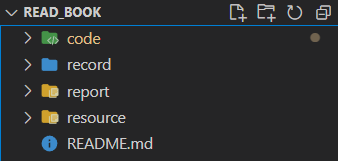
\includegraphics[width=0.35\columnwidth]{figures/fileopen.png}
              \caption{IDE打开文件夹(图为Visual Studio Code)}
          \end{figure}
    \item 打开 code-database-Databaseconn.py, 修改数据库host, user, password为你自己的信息

          \begin{figure}[H]
              \centering
              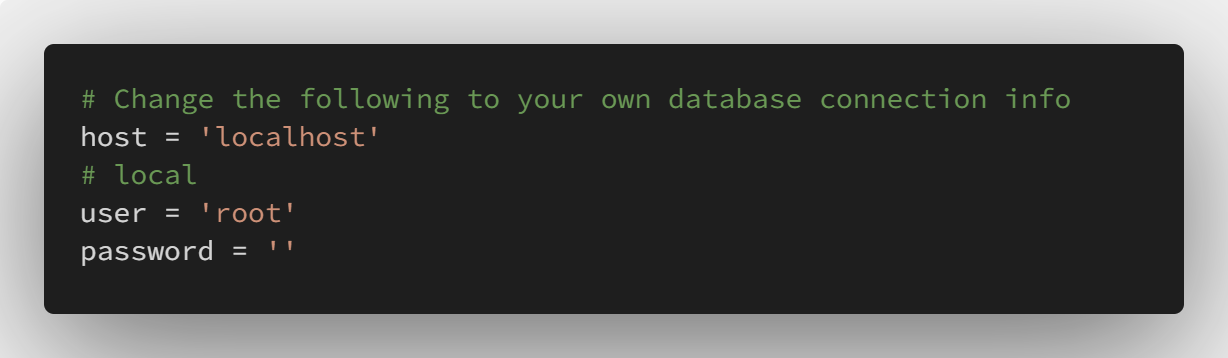
\includegraphics[width=0.9\columnwidth]{figures/sql.png}
              \caption{修改数据库信息}
          \end{figure}
    \item 直接运行code文件夹下的main.py
          \begin{figure}[H]
              \centering
              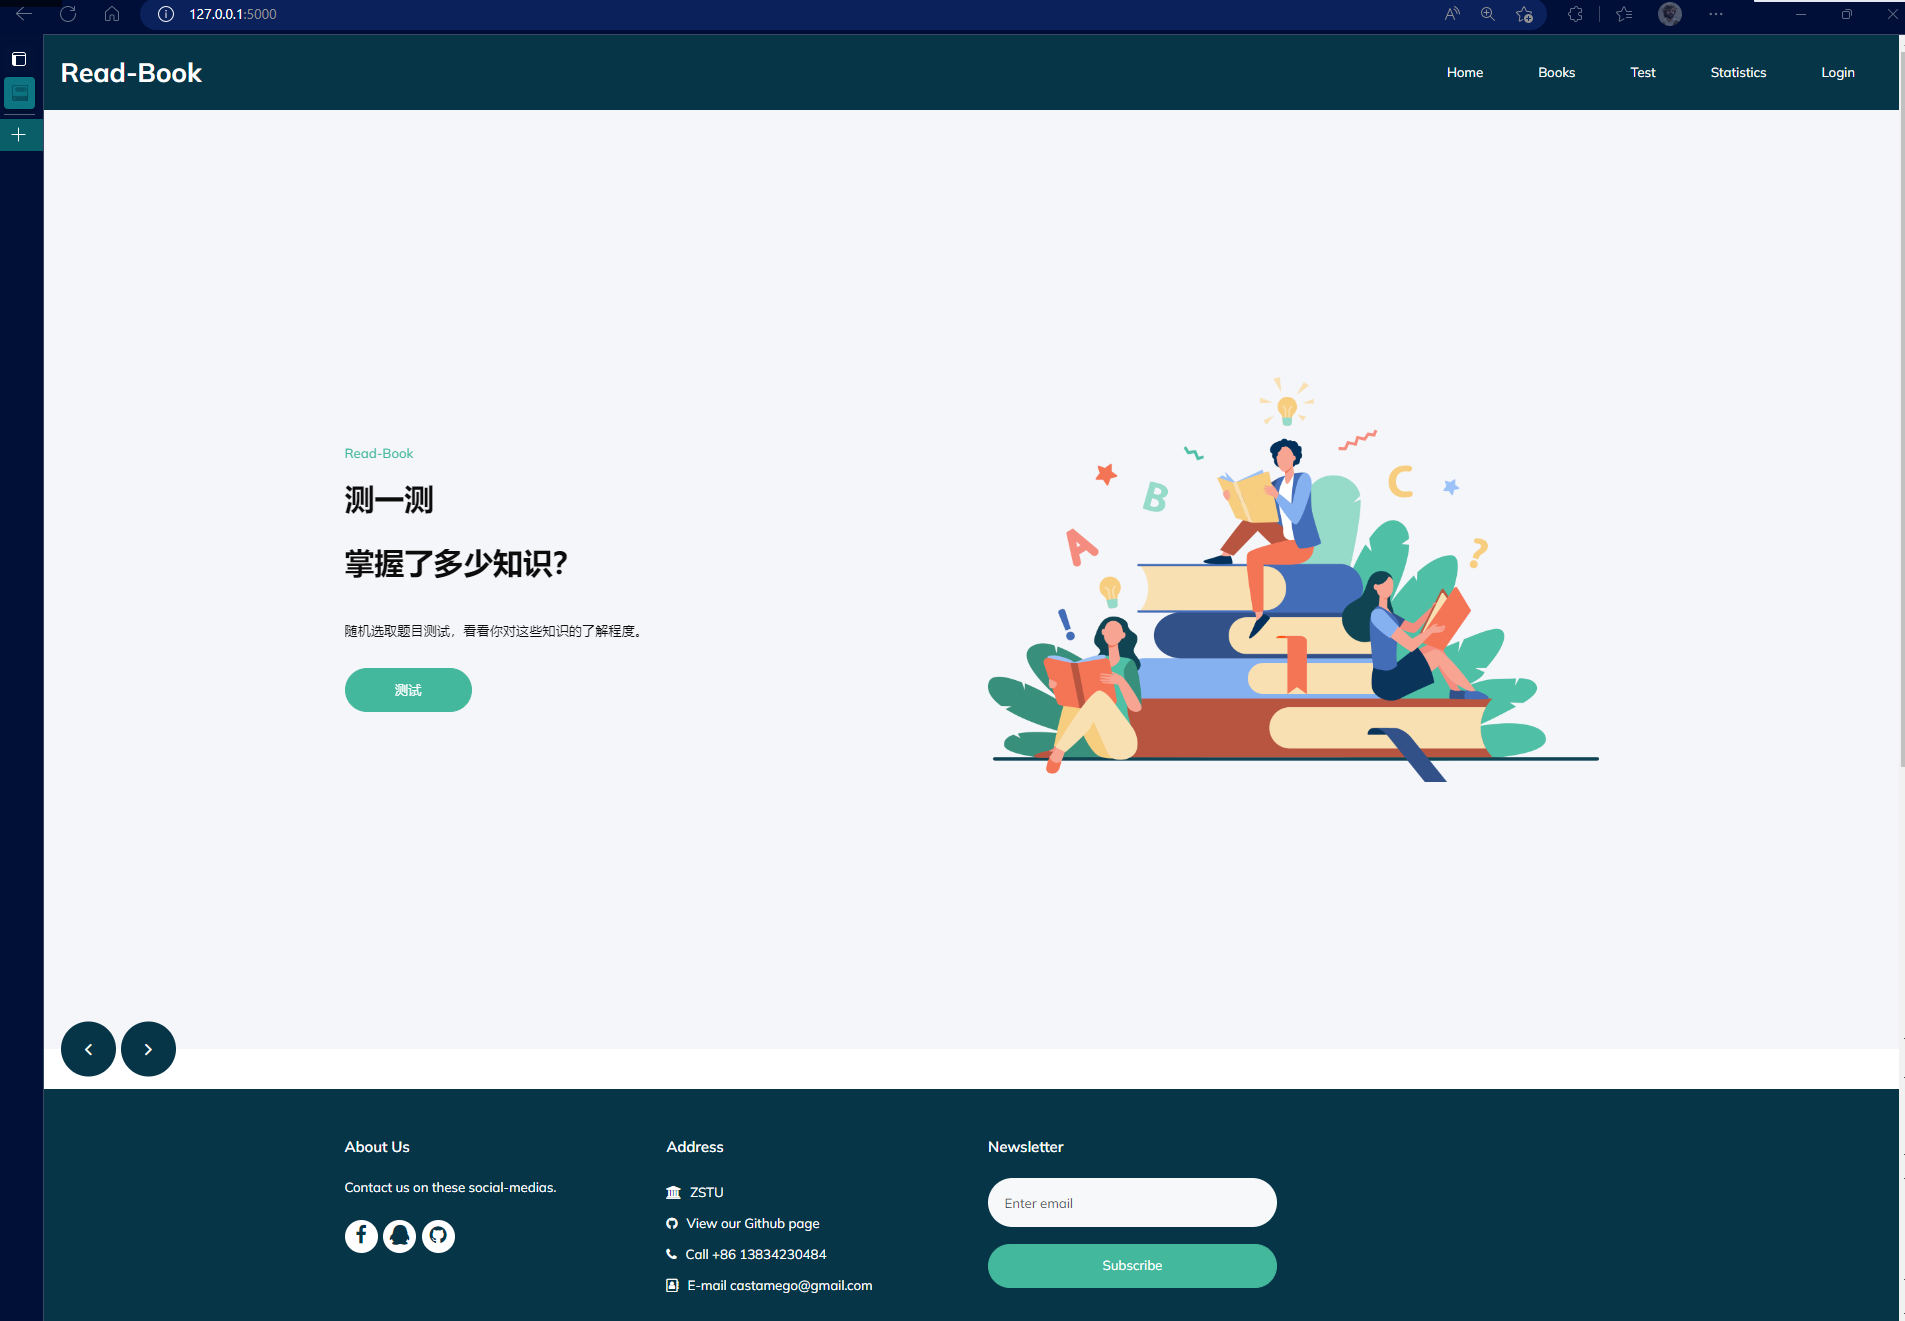
\includegraphics[width=1\columnwidth]{figures/demo.png}
              \caption{运行成功~可以开香槟了}
          \end{figure}
\end{enumerate}

\end{document}